\section{Mise en place du \textit{front-end}}

\begin{frame}{Mise en place du \textit{front-end}}
  \begin{block}{Les aspects du développement \textit{front-end}}
    \begin{itemize}
    \item La structure avec HTML.
    \item Le style avec CSS.
    \item Le comportement avec le Javascript.
    \end{itemize}
  \end{block}
\end{frame}

\subsection{HTML}
\begin{frame}{Structure HTML du projet}
  \begin{figure}
  \begin{center}
    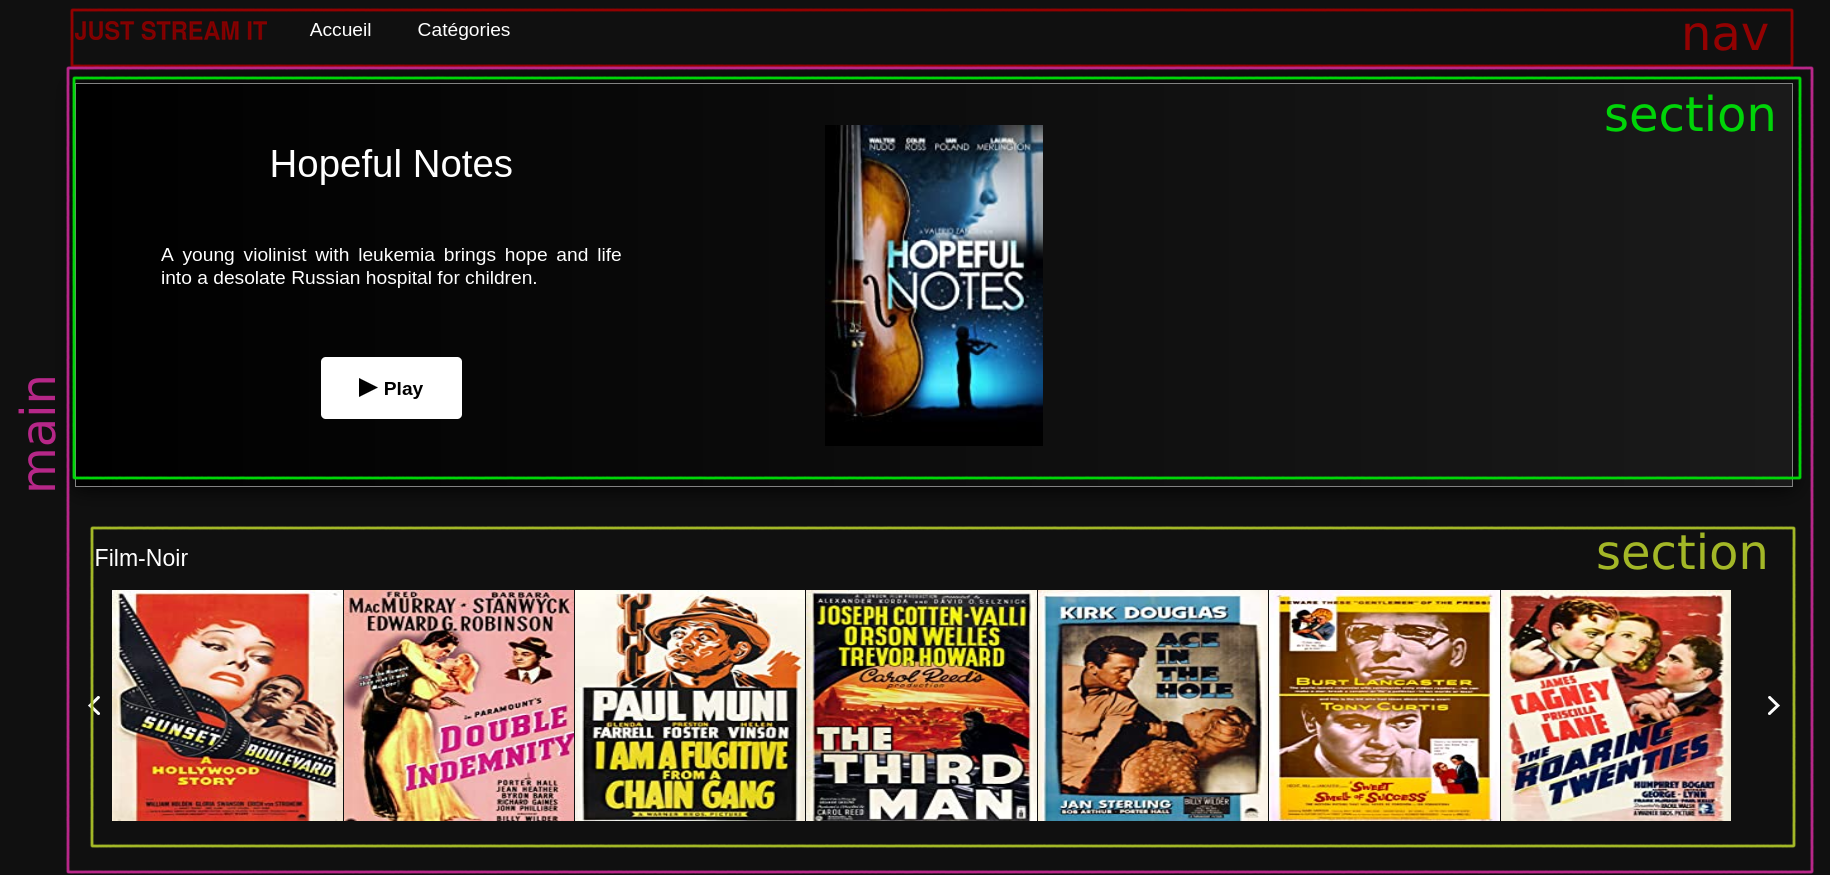
\includegraphics[scale=0.15]{img/html.png}
  \end{center}
  \caption{Éléments HTML de la page d'accueil}
  \end{figure}
\end{frame}

\subsection{CSS}

\begin{frame}[fragile]{Un CSS maintenable et \textit{scalable} avec SASS}  
  \begin{block}{Organisation}
    \begin{itemize}
    \item Séparation du style sur plusieurs fichiers
    \item Application du \textit{pattern} 7-1
    \end{itemize}
  \end{block}

  \begin{minted}{sass}
    @import 'base/reset';
    @import 'abstracts/mobile';
    @import 'themes/theme';
    @import 'layout/nav';
    @import 'pages/home';
    @import 'components/buttons';
    @import 'components/best_movie';                                                                                                                 @import 'components/category';
    @import 'components/movie_info';
  \end{minted}

\end{frame}

\begin{frame}[fragile]{Un CSS \textit{responsive}}
  \begin{block}{aze}
    \begin{itemize}
    \item Approche \textit{Mobile first} lors du développement.
    \item Utilisation d'une mixin SCSS pour gérer les \textit{media queries}.
    \end{itemize}
  \end{block}
  
  \begin{minted}[mathescape]{sass}
    @mixin for-mobile {
      @media screen and (max-width: 599px) {
        @content
      }
    }
  \end{minted}
\end{frame}

\begin{frame}[fragile]{Un CSS \textit{responsive}: exemple}
  
  \begin{minted}[mathescape]{sass}
    @include for-mobile {
        position: fixed;
        margin: 0;
        top: 0;
        left: 0;
        width: 100%;
        min-width: 0;
        height: 100%;
        max-height: 100%;
    }
  \end{minted}
\end{frame}

\begin{frame}[fragile]{Un CSS organisé avec la méthode BEM}
  % les autres méthodologie
  % pourquoi BEM ?
  % mise en place de BEM
  
  \begin{block}{La méthode BEM}
    \begin{itemize}
    \item Permet d'organiser le CSS.
    \item Extensible au SCSS.
    \item Signifie {\color{red}{\textit{Block}}} - {\color{violet}{\textit{Element}}} - {\color{teal}{\textit{Modifier}}}.
    \item Propose un formatage dans le choix des noms de classe CSS d'un projet.
    \end{itemize}    
  \end{block}

  \begin{block}{Un exemple de formatage}
    \textsc{\color{red}{nom\_bloc} \color{violet}{\_ \_ nom\_element} \color{teal}{- - nom\_modifier}}
  \end{block}
\end{frame}

\begin{frame}[fragile]{Le BEM appliqué au SASS}
  \begin{block}{En SASS}
    \scriptsize
    \begin{minted}{sass}
      .best_movie {
        &__title {
          &--blue {}
        }
      }
    \end{minted}
  \end{block}

  \begin{block}{En CSS}
    \scriptsize
    \begin{minted}{sass}
      .best_movie {}
      .best_movie best_movie__title {}
      .best_movie best_movie__title best_movie__title--blue {}
    \end{minted}
  \end{block}
\end{frame}

\subsection{Javascript}
\begin{frame}{Structure du code Javascript}
\end{frame}

\begin{frame}{Utilisation de NPM}
  % webpack
  % on peut s'en passer !
  % avantages / inconvénient
\end{frame}

\begin{frame}{Récupération des informations \textit{via} l'API}
\end{frame}

\begin{frame}{Génération HTML des catégories}
\end{frame}

\begin{frame}{Mise en place du carrousel}
\end{frame}

\begin{frame}{Gestion de la modale}
\end{frame}
